% !TEX root = ./main.tex

\section{Numerics}
\label{sec:numerics}
\subsection{Flux Reconstruction Method}

What follows is an overview of the flux reconstruction (FR) framework. We start the discussion with the solution of the advection-diffusion equation in one dimension using the FR approach to illustrate the peculiarities of the method. We then proceed to briefly explain how conservation equations can be solved in multiple dimensions. The NS equations are a set of coupled conservation equations in multiple dimensions, so the extension of the FR methodology to them is straightforward. The detailed description of the algorithm used in HiFiLES is given by Castonguay et al. \cite{castonguay2011}.

\subsubsection{Solution of the Advection Equation in One Dimension using the FR Approach}

Consider the one-dimensional conservation law
\begin{equation}
\label{eq:cons}
\frac{\partial u}{\partial t} + \frac{\partial f}{\partial x} = 0
\end{equation}

in domain $\Omega$, where $x$ is the spatial coordinate, $t$ is time, $u$ --the \emph{solution}-- is a scalar function of $x$ and $t$, and $f$ --the \emph{flux}-- is a scalar function of $u$. Note that by letting $f = f(u,\frac{\partial u}{\partial x})$, Equation~\ref{eq:cons} becomes a model of the Navier-Stokes equations.

Let us partition the domain $\Omega = [x_1,x_{N+1})$ into $N$ non-overlapping elements with 
interfaces at $x_1<x_2<...<x_{N+1}$. Then,
\begin{equation}
\Omega = \bigcup^N_{n=1} \Omega_n
\end{equation}
and $\Omega_n = [x_n,x_{n+1})$ for $n = 1,...,N$.

To simplify the implementation, let us map each of the physical elements $\Omega_n$ to a standard 
element $\Omega_s=[-1,1)$ with the function $\Theta_n(\xi)$, where
\begin{equation}
x = \Theta_n(\xi) = \l( \frac{1-\xi}{2} \r) x_n + \l(\frac{1+\xi}{2}\r) x_{n+1} 
\end{equation}

With this mapping, the evolution of $u$ within each $\Omega_n$ can be determined with the following 
transformed conservation equation
\begin{equation}
\frac{\partial \hat{u}}{\partial t} + \frac{1}{J_n}\frac{\partial \hat{f}}{\partial \xi} = 0
\end{equation}
where
\begin{equation}
\hat{u} = u(\Theta_n(\xi),t) \text{ in } \Omega_n
\end{equation}
\begin{equation}
\hat{f} = f(\Theta_n(\xi),t) \text{ in } \Omega_n
\end{equation}
\begin{equation}
J_n = \frac{\partial x}{\partial \xi} \bigg|_{\Omega_n}
\end{equation}

Now, introduce polynomials of degree $p$, $\hat{u}^\delta$ and $\hat{f}^\delta$, to 
approximate the exact values $\hat{u},\hat{f}$, respectively. We can write these polynomials as
\begin{equation}
\hat{u}^\delta = \sum_{i=1}^{N_s} \hat{u}_i^\delta l_i(\xi)
\end{equation}
\begin{equation}
\hat{f}^\delta = \sum_{i=1}^{N_s} \hat{f}_i^\delta l_i(\xi)
\end{equation}
where $N_s$ is the number of solution points, $\hat{u}_i^\delta$ is the current value of the 
solution approximation function at the $i^\text{th}$ \emph{solution point} in the reference element, 
$\hat{f}_i^\delta$ is the current value of the flux approximation function at the $i^\text{th}$ 
\emph{flux point} in the reference element, $l_i$ is the Lagrange polynomial equal to $1$ at the 
$i^\text{th}$ solution point and $0$ at the others, and $\delta$ denotes that the function is an 
approximation.

Note that the piecewise polynomials might not be continuous (or $C^0$) accross the interfaces. In the 
Flux Reconstruction approach, the flux used in the time advancement of the solution is made $C^0$ 
by introducing flux correction functions.

This can be achieved by finding interface solution values at each element boundary and then correcting the 
solution. Let $\hat{u}_L^{\delta I}$ and $\hat{u}_R^{\delta I}$ be the interface solution values at left and right 
boundaries of some element, respectively. $\hat{u}_L^{\delta I}$ and $\hat{u}_R^{\delta I}$ can be found with a Riemann solver for Discontinuous-Galerkin (DG) methods\cite{hesthaven2007}. Then, select solution correction functions $g_L$ and 
$g_R$ such 
that
\begin{equation}\label{eq:condition}
g_L(-1) = 1 \;,\; g_L(1) = 0
\end{equation}
\begin{equation}
g_R(-1) = 0 \;,\; g_R(1) = 1
\end{equation}
and let
\begin{equation}
\hat{u}^C = \hat{u}^\delta + (\hat{u}^{\delta I}_L - \hat{u}^\delta_L) g_L + (\hat{u}^{\delta I}_R 
- \hat{u}^\delta_R) g_R
\end{equation}
where superscript $C$ denotes the function is corrected, and $\hat{u}^\delta_L$, $\hat{u}^\delta_R$ 
represent the solution approximation evaluated at the left and right boundaries.

Using the values of $\hat{u}^\delta_i$ and $\frac{\partial \hat{u}^C}{\partial \xi}|_{\xi_i}$ we then find 
$$\hat{f}_i^\delta = \hat{f}\l(\hat{u}^\delta_i,\frac{1}{J_n}\frac{\partial \hat{u}^C}{\partial \xi}\bigg|_{\xi_i}\r) \;\; \text{in element } \Omega_n$$
We can proceed in a similar fashion to correct the flux to obtain
\begin{equation}
\hat{f}^C = \hat{f}^\delta + (\hat{f}^{\delta I}_L - \hat{f}^\delta_L) h_L + (\hat{f}^{\delta I}_R 
- \hat{f}^\delta_R) h_R
\end{equation}
where $h_R$ and $h_L$ are right and left flux correction functions satisfying the same boundary 
conditions as $g_R$ and $g_L$, respectively, and $\hat{f}_L^{\delta I}$ and $\hat{f}_R^{\delta I}$ are the interface fluxes found via a Riemann solver. Note that if the flux corresponds to linear advection, correcting the solution and correcting the flux are equivalent steps.

The solution can then be advanced at each solution point. In semi-discrete form, this is
\begin{equation}\label{eq:semidiscrete}
\frac{d \hat{u}_i^\delta}{d t} = - \frac{\partial \hat{f}^c}{\partial \xi}(\xi_i)
\end{equation}

The FR scheme can be made provably stable for the linear advection-diffusion equation by selecting special types of correction functions\cite{castonguay2013}. In general, these correction functions are polynomials of degree $p+1$ so both sides in Equation~\eqref{eq:semidiscrete} are quantities related to polynomials of order $p$ --for consistency\cite{huynh2007}.

Vincent et al. \cite{vincent2011new} have shown that in the case of the 1-dimensional, linear advection equation, the Flux Reconstruction approach can be proven to be stable for a specific family of correction functions parameterized by a scalar called $c$. In addition, they showed that by selecting specific values of $c$ it is possible to recover a particular nodal DG and Spectral Difference (SD) methods plus a FR scheme that was previously found to be stable by Huynh\cite{huynh2007flux}.

%The final paper, for completeness, will include a description of the Flux Reconstruction\cite{vincent2011new} approach and the reasoning behind using the Energy-Stable version. A thorough description of the steps taken in the calculation of the residual for the 3D NS Equations will be included.


\subsection{Unstructured Mesh Treatment}
Extension to multiple dimensions requires formulating multi-dimensional interpolation functions and correction functions that satisfy boundary conditions equivalent to those in Equation~\eqref{eq:condition} for each type of element.

Interpolation bases for quadrilaterals and hexahedra can be obtained via tensor products of the 1-dimensional interpolation basis. More concretely, in HiFiLES, we discretize the solution in 3-dimensions in the following way
\begin{equation}
{\bf \hat{u}}^\delta(\xi,\eta,\zeta) = \sum_{i=1}^{p+1} \sum_{j=1}^{p+1} \sum_{k=1}^{p+1}
{\bf \hat{u}}^\delta_{i,j,k} l_i(\xi) l_j(\eta) l_k(\zeta)
\end{equation}
where $i$, $j$, $k$ index the solution points along the $\xi, \eta, \zeta$ directions, respectively. The flux is discretized similarly.

The interpolation basis for triangles are described in detail by Castonguay et al. \cite{castonguay2012new} and Williams et al. \cite{williams2013tri}. The formulation for tetrahedra is detailed by Williams et al. \cite{williams2013tet}.

The extension of interpolation polynomials to prisms is obtained via tensor products of the 1-dimensional basis with the triangular basis\cite{castonguay2011}. 

In general, the boundary conditions for the correction functions in multiple dimensions can be formulated as
\begin{equation}\label{eq:genConstraint}
{\bf h}_i( \vec{\xi}_j)\cdot {\bf n}_j = \delta_{ij}
\end{equation}
where ${\bf h}_i$ is the vector of correction functions associated with interface point $i$, $\vec{\xi}_j$ is the location vector of the $j^\text{th}$ interface point, ${\bf n}_j$ is the outward unit normal at interface point $j$, and $\delta_{ij}$ is the Kronecker delta. Interface points are located on the boundary of an element.

One of the challenges in the FR approach is finding correction functions that not only satisfy Equation~\eqref{eq:genConstraint} but also guarantee stability in the linear advection-diffusion case. Correction functions that guarantee such stability exist for 1-dimensional segments\cite{vincent2011new}, triangles\cite{castonguay2012new,williams2013tri}, and tetrahedra\cite{williams2013tet}. FR schemes with these correction functions comprise the ESFR family of schemes.

Although formal proofs of stability for the linear advection equation do not exist yet for quadrilaterals, hexahedra, and prisms, it has been observed that the tensor products of provably stable correction functions used in these elements maintain stability. In addition, as of now HiFiLES does not have an implementation for pyramidal elements, mostly because of the challenges involved in finding the respective correction functions that guarantee stability. Nevertheless, a suggested approach to find such correction functions has been presented by Jameson\cite{jameson2011advances}.


%\subsection{Time Stepping and p-multigrid}
%Explicit RK4 with ability to use multigrid\cite{fidkowski2005p} and dual time-stepping\cite{Jameson1991DualTime} for implicit time advancement.

%\subsection{Stabilization Techniques}

\subsection{Large Eddy Simulation Models}\label{lesmodels}

In order to resolve all the scales of motion in a high Reynolds number turbulent flow, the computational mesh would have to be impractically fine.
A practical solution is to employ the Large Eddy Simulation (LES) formulation, which only resolves the larger scales of motion and thus allows for the use of coarser meshes.
The effect of the unresolved or subgrid-scale (SGS) dynamics on the solution is accounted for by an SGS model for the \emph{subgrid-scale stress} $\tau_{ij}$, which is added to the viscous stress tensor $\sigma_{ij}$ given by (\ref{sigma}):
%
\begin{eqnarray}\label{tausgs}
\sigma_{ij} &&= 2 \mu S^d_{ij} + \tau_{ij},\\
S^d_{ij} &&= \frac 1 2 \l( \frac{\partial u_i}{\partial x_j} + \frac{\partial u_j}{\partial x_i} - \frac{2}{3} \delta_{ij}\frac{\partial u_k}{\partial x_k} \r).
\end{eqnarray}
%
The standard Smagorinsky model\cite{smagorinsky1963} is available in HiFiLES:
%
\begin{eqnarray}\label{smag}
\tau_{ij} &&= 2 \rho \nu_t S^d_{ij}, \\
\nu_t &&= C_S^2 \bigtriangleup^2 | S^d |,\\
| S^d | &&= \sqrt{2 S^d_{ij} S^d_{ij}},
\end{eqnarray}
%
where $\nu_t$ is the eddy viscosity, $C_S = 0.1$ is the Smagorinsky coefficient and $\bigtriangleup$ is the filter width.
In HiFiLES the filter width is given by (in 3D):
%
\begin{equation}
\bigtriangleup = \alpha (\text{vol})^{1/3},
\end{equation}
%
where $\alpha \geq 1$ is a user-defined scaling factor and vol is the element volume.
HiFiLES also includes the Wall-Adapting Local Eddy-Viscosity (WALE) model~\cite{nicoud1999} and the Similarity model~\cite{bardina1980}.
The Similarity model incorporates a low-pass filtering operator, for which several choices are available in HiFiLES: a discrete Gaussian filter\cite{lodato2012b}, a high-order commuting Vasilyev-type filter\cite{vasilyev1998,vasilyev2001} and a modal Vandermonde-type filter\cite{blackburn2003}.
The modal filter is able to be used on unstructured tetrahedral meshes.
For details of these operators, see Lodato, Castonguay and Jameson~\cite{lodato2012b} and Bull and Jameson~\cite{bull2013a}.
Also available is the option to combine the similarity model with the Smagorinsky or WALE model to form a mixed SGS model.
The WALE-similarity mixed (WSM) model, first proposed by Lodato et al.~\cite{lodato2009}, was used in simulations of the flow over a square cylinder (see Section \ref{sqcyl}).
%Finally, a Spectral Vanishing Viscosity (SVV) model is available.
%Instead of adding a model term, the SVV method applies one of the above mentioned filters directly to the solution in order to damp the small scales or high-order modes~\cite{karamanos2000}.

\subsection{Computing Architecture and Scalability}
%The final paper will include a description of how HiFiLES is designed for a multi-GPU environment. Studies performed without filtering or SGS modeling in \cite{castonguay2011}. 

The HiFiLES code has been designed to work on multi-CPU as well as multi-CPU-GPU platforms. The Flux Reconstruction method in its current form with explicit time-stepping has a great potential for parallelization. Since the solution points are not explicitly shared between elements, most of the computations are element-local enabling an efficient use of shared memory on GPUs. Also, several computations are independent for each solution point and the highly parallelizable nature of GPUs becomes very useful. A detailed description of the parallelization of the FR method, along with scalability and performance analysis has been performed in \cite{castonguay2011}.

\subsection{Shock capturing and Stabilization Models}

We use the method of concentration described in \cite{abhishekshockcapture} for detecting shocks on meshes with quadrilateral elements. We are still in the process of extending the method of concentration to triangles and are currently using Persson and Peraire's method \cite{Persson06} \cite{Persson13} for the same. We have explored both selective addition of artificial viscosity as well as modal order reduction for capturing the detected shocks effectively. Persson and Peraire have used this shock capturing tool as a stabilization method as well in their turbulence calculations. Here we show a viscous case on quads using concentration method (reproduction of the result in \cite{abhishekshockcapture}) and an inviscid case on triangles using Persson and Peraire's method.

\begin{figure}
\centering
\begin{minipage}[t]{.5\textwidth}
  \centering
  %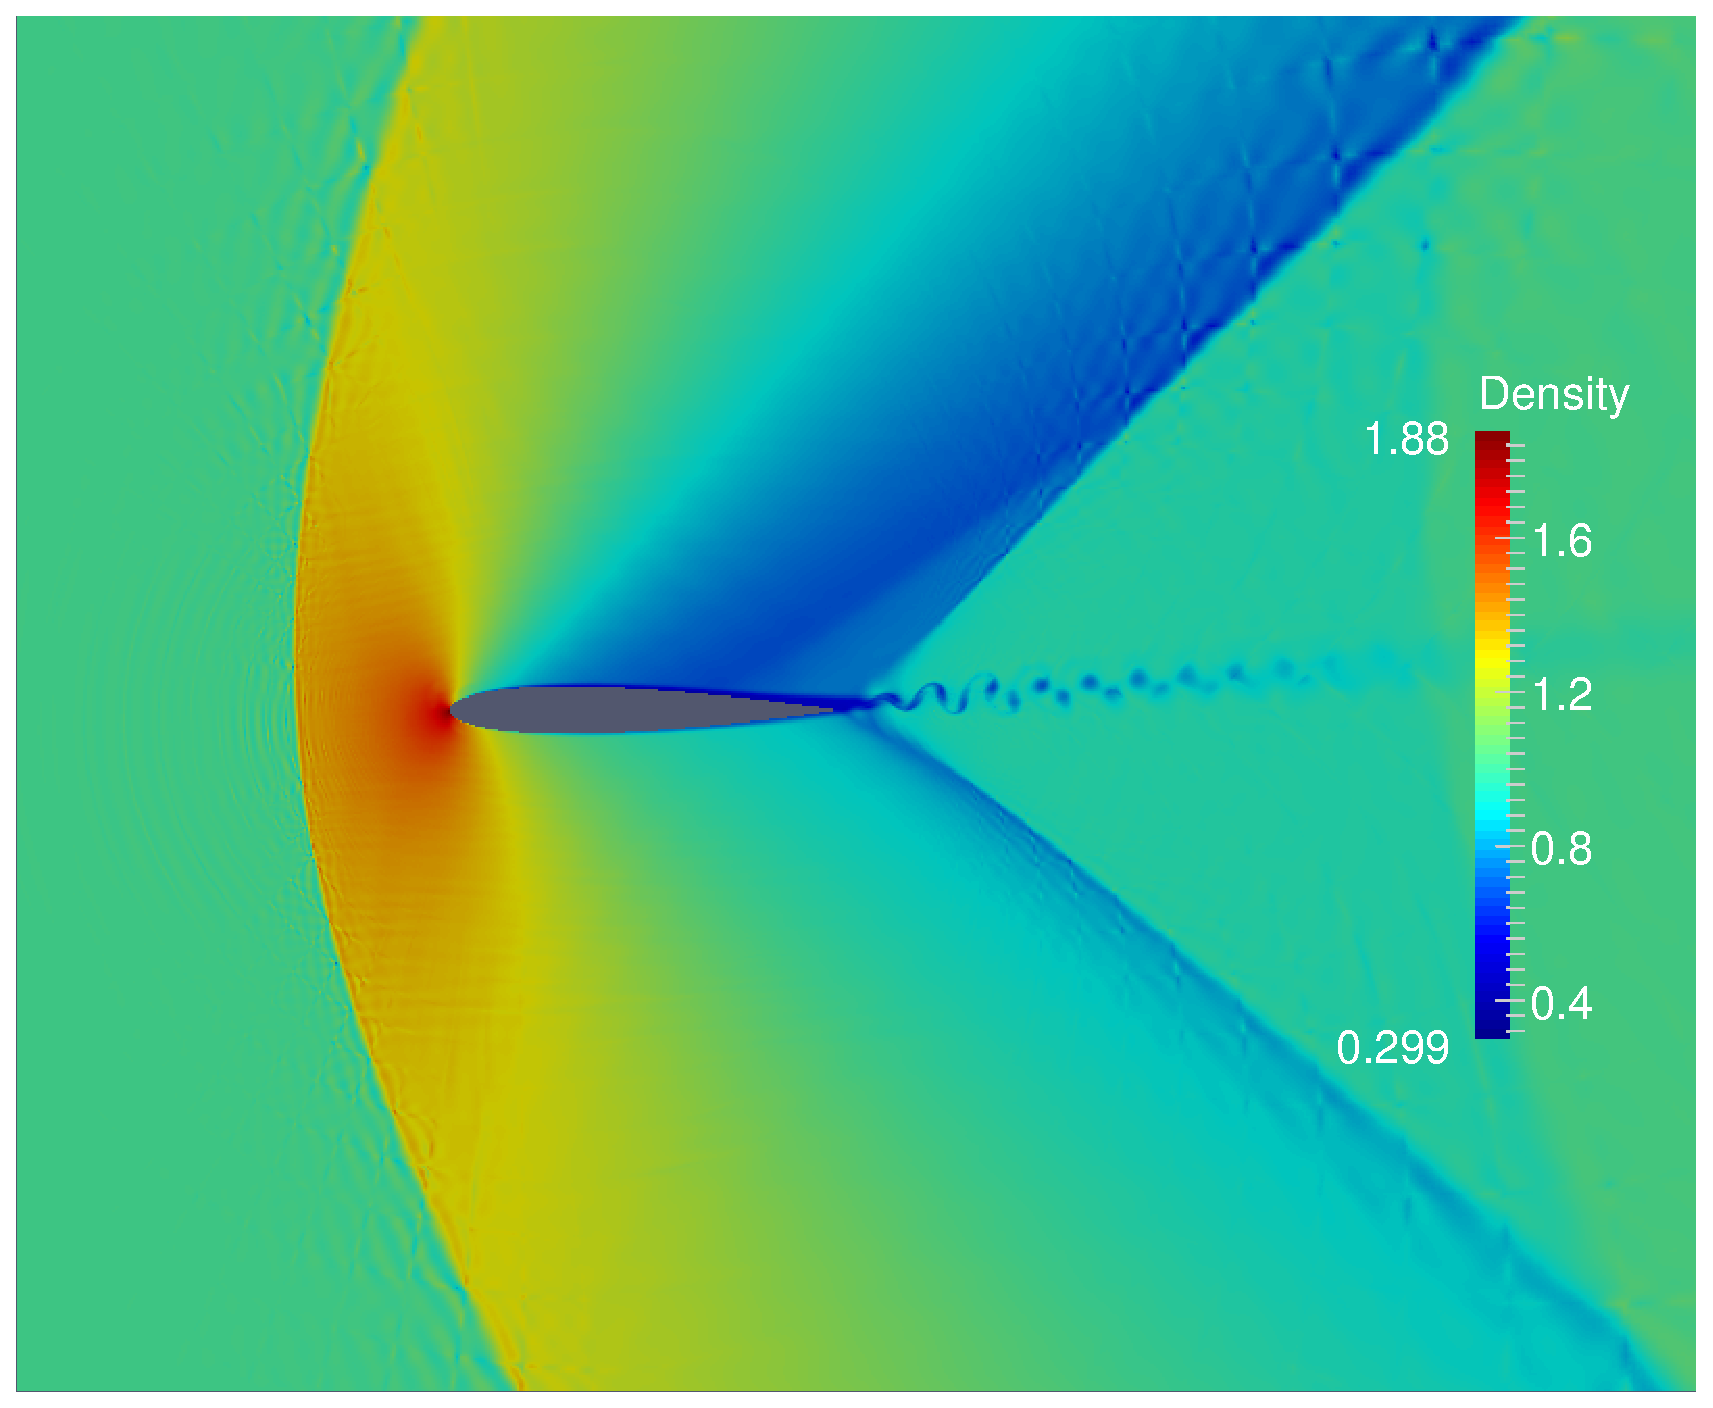
\includegraphics[width=.85\linewidth]{./figures/density-t1050010-jet}
  \captionof{figure}{density contours respectively for viscous flow at M = 1.2 over a NACA 0012 airfoil at 5$^{\circ}$ AoA with polynomial order 6 (49 points in each element)}
  \label{fig:visM1pt2-density}
\end{minipage}%
\begin{minipage}[t]{.5\textwidth}
  \centering
  %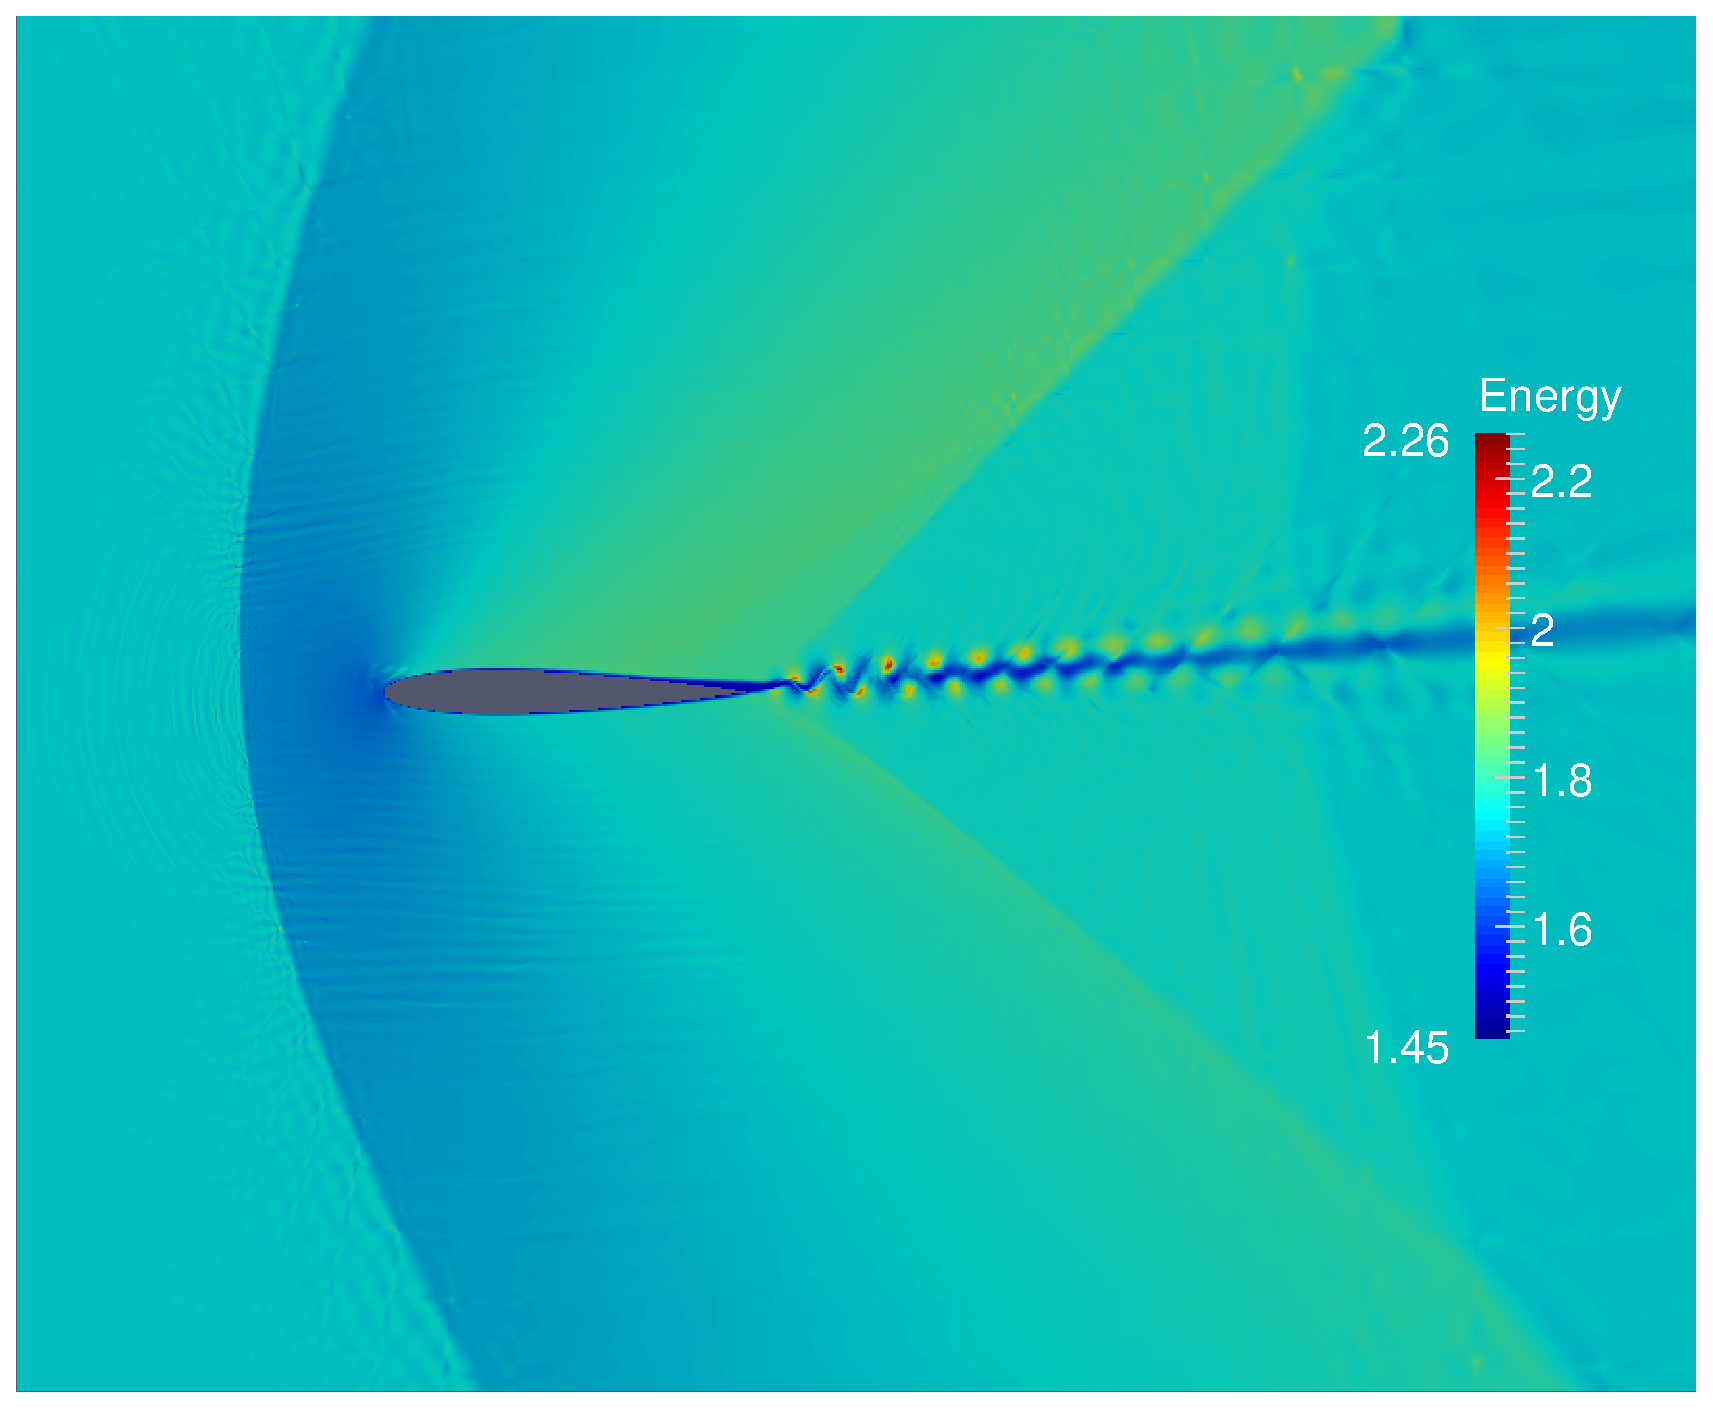
\includegraphics[width=.85\linewidth]{./figures/energy-t1050010-jet}
  \captionof{figure}{Energy contours}
  \label{fig:visM1pt2-energy}
\end{minipage}
\end{figure} 

\begin{figure}[h] \tt
\centering
%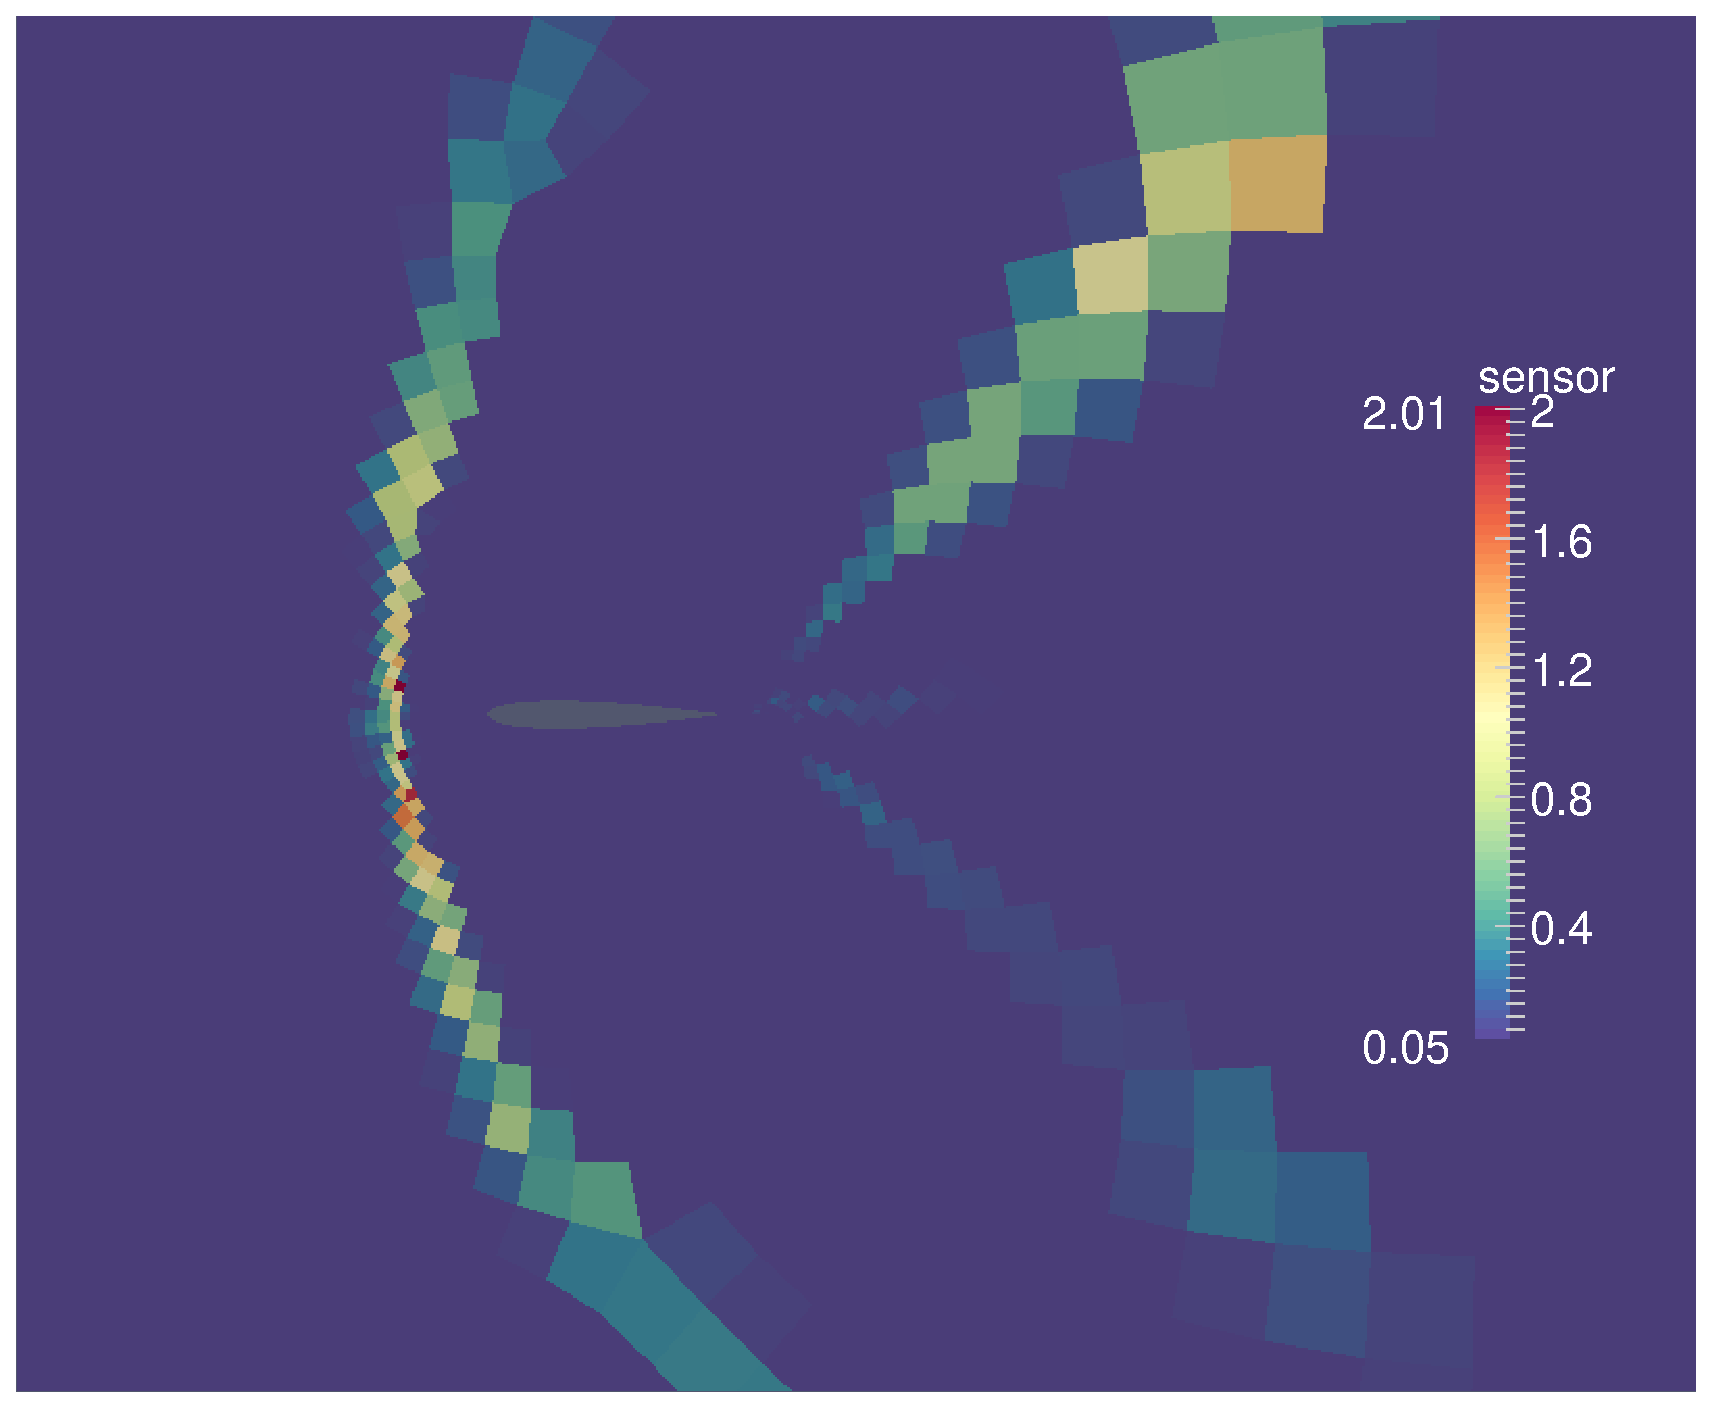
\includegraphics[angle=0, scale = 0.55]{./figures/sensor-t1050010-spectral} \\
\caption{Figure shows the elemental shock "sensor" for the M = 1.2 viscous case shown in figure ~\ref{fig:visM1pt2-density}. The shock sensor is just the maximum value of the enhanced kernel in each element}
\label{fig:sensor}
\end{figure}

\begin{figure}[h] \tt
\centering
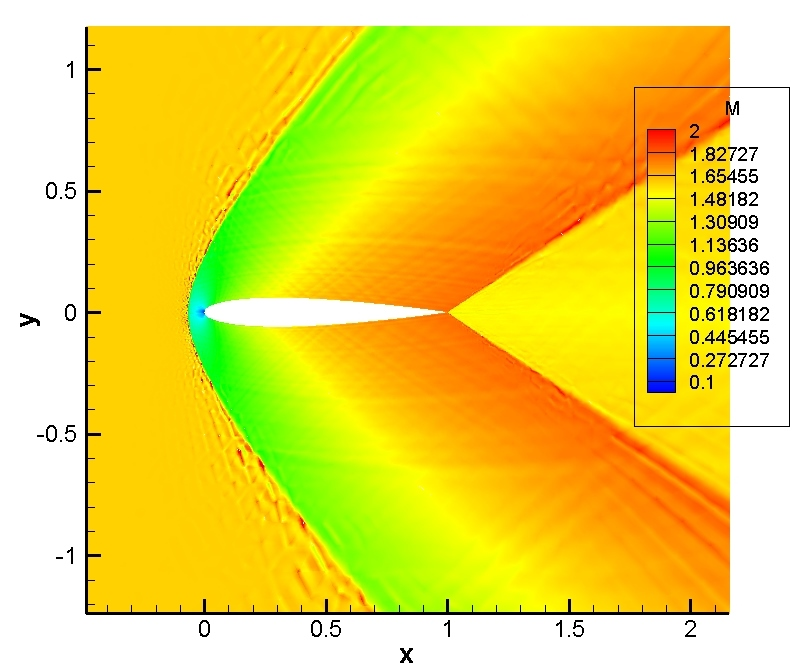
\includegraphics[angle=0, scale = 0.68]{./figures/M1pt6order3-inv-720ktime-mach.jpg} \\
\caption{Mach contours for inviscid flow over Naca0012 at M = 1.6 and AoA = $0^{\circ} $ on a triangle-mesh using Persson and Peraire's method and using artificial viscosity}
\label{fig:inv_mach}
\end{figure}

\begin{figure}
\centering
\begin{minipage}[t]{.55\textwidth}
  \centering
  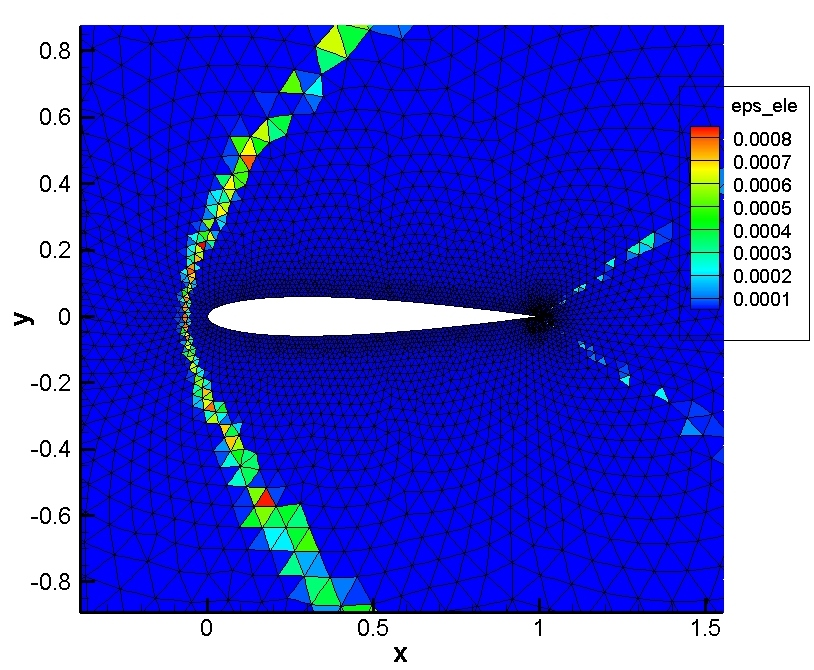
\includegraphics[width=.85\linewidth]{./figures/M1pt6-inv-av-ele-mesh}
  \captionof{figure}{Element-wise AV co-efficients for the inviscid M 1.6 case}
  \label{fig:AV-ele}
\end{minipage}%
\begin{minipage}[t]{.55\textwidth}
  \centering
  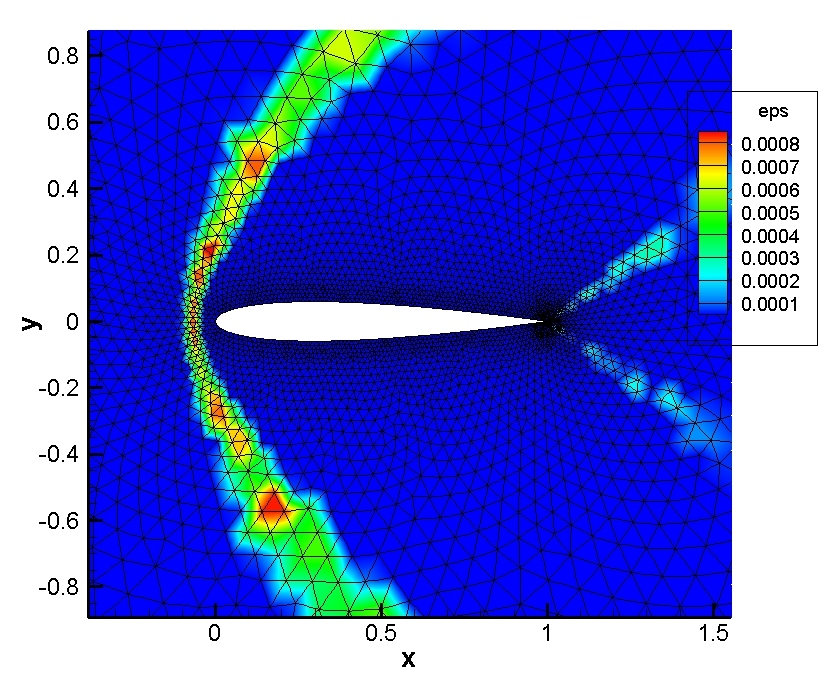
\includegraphics[width=.85\linewidth]{./figures/M1pt6-inv-av-mesh}
  \captionof{figure}{AV co-efficients with continuity enforcement}
  \label{fig:AV-cont}
\end{minipage}
\end{figure} 


\subsection{Spalart-Allmaras (SA) Turbulence Model and Negative $\tilde\nu$ Modification}
The one equation SA turbulence model is one of the more commonly used turbulence models used to solve attached and moderately separated aerodynamic flows \cite{spalart1992one}. The added equation directly solves for turbulent eddy viscosity via advection, diffusion, production and dissipation. A modified form of the equation can be written as \cite{burgess2012robust,oliver2008high,moro2011navier}:
\begin{align}
	\frac{\partial}{\partial t}(\rho\tilde\nu) + \nabla\cdot(\rho\tilde\nu\boldsymbol{u}) = c_{b_1}\tilde S \rho\nu\psi + \frac{1}{\sigma}\left[\nabla\cdot((\mu + \mu\psi)\nabla\tilde\nu) + c_{b_2}\rho\nabla\tilde\nu\cdot\nabla\tilde\nu\right] - c_{w_1}\rho f_w \left(\frac{\nu\psi}{d}\right)^2
\end{align}

where $\tilde\nu$ is a modified version of the kinematic eddy viscosity and $\nu$ is the kinematic viscosity. The other variables are defined as,

\begin{align}
	 \mu_t =
	  \begin{cases}
	   \rho\tilde\nu f_{v_1} & \text{if } \tilde\nu \ge 0 \\
	   0       & \text{if } \tilde\nu < 0
	  \end{cases}
	  \quad \mbox{where} \quad f_{v_1} = \frac{\left(\frac{\rho\tilde\nu}{\mu}\right)^3}{\left(\frac{\rho\tilde\nu}{\mu}\right)^3 + c_{v_1}^3}
\end{align}

\begin{align}
	\tilde S &=
	\begin{cases}
	   S + \bar S & \text{if } \bar S \ge -c_{v_2}S \\
	   S + \frac{S(c_{v_2}^2 S + c_{v_3}\bar S)}{(c_{v_3} - 2c_{v_2})S - \bar S} & \text{if } \bar S \le -c_{v_2}S
	\end{cases}
\end{align}
\begin{align}
	S &= \sqrt{\boldsymbol{\omega}\cdot\boldsymbol{\omega}}
	\qquad \bar S = \frac{(\nu\psi)^2 f_{v_2}}{\kappa^2 d^2} \\
	f_{v_2} &= 1 - \frac{\psi}{1 + \psi f_{v_1}}
\end{align}

\begin{align}
	f_w &= g\left[\frac{1 + c_{w_3}^6}{g^6 + c_{w_3}^6}\right]^{1/6} 
	\qquad g = r + c_{w_2}(r^6 - r) 
	\qquad r = \frac{\nu\psi}{\tilde S \kappa^2 d^2}
\end{align}

where S is the magnitude of vorticity, d is the closest distance to a wall, $c_{b1} = 0.1355$, $\sigma = \frac{2}{3}$, $c_{b2} = 0.622$, $K = 0.41$, $\text{Pr}_t = 0.9$, $c_{v1} = 7.1$, $c_{v2} = 0.7$, $c_{v3} = 0.9$, $c_{w1} = \frac{c_{b1}}{K^2} + \frac{(1+c_{b2})}{\sigma}$, $c_{w2} = 0.3$, $c_{w3} = 2$.\\

The diffusion term, $\nabla\cdot(\rho\tilde\nu\boldsymbol{u})$, may become discontinuous in the first derivative leading to oscillations in high-order polynomials. This can lead to large negative values of the modified eddy viscosity term, $\tilde\nu$, significant enough to cause an unbounded solution. To prevent this, the following modification is introduced \cite{moro2011navier}.
\begin{align}
	\psi &=
	\begin{cases}
	   0.05log(1.0 + e^{(20.0\chi)}) & \text{if } \chi \le 10.0 \\
	   \chi & \text{if } \chi > 10.0
	\end{cases} \\
	\chi &= \frac{\tilde\nu}{\nu}
\end{align}
